\documentclass{article}
\usepackage[backend=biber,natbib=true,style=alphabetic,maxbibnames=50]{biblatex}
\addbibresource{/home/nqbh/reference/bib.bib}
\usepackage[utf8]{vietnam}
\usepackage{tocloft}
\renewcommand{\cftsecleader}{\cftdotfill{\cftdotsep}}
\usepackage[colorlinks=true,linkcolor=blue,urlcolor=red,citecolor=magenta]{hyperref}
\usepackage{amsmath,amssymb,amsthm,enumitem,float,graphicx,mathtools,tikz}
\usetikzlibrary{angles,calc,intersections,matrix,patterns,quotes,shadings}
\allowdisplaybreaks
\newtheorem{assumption}{Assumption}
\newtheorem{baitoan}{}
\newtheorem{cauhoi}{Câu hỏi}
\newtheorem{conjecture}{Conjecture}
\newtheorem{corollary}{Corollary}
\newtheorem{dangtoan}{Dạng toán}
\newtheorem{definition}{Definition}
\newtheorem{dinhly}{Định lý}
\newtheorem{dinhnghia}{Định nghĩa}
\newtheorem{example}{Example}
\newtheorem{ghichu}{Ghi chú}
\newtheorem{hequa}{Hệ quả}
\newtheorem{hypothesis}{Hypothesis}
\newtheorem{lemma}{Lemma}
\newtheorem{luuy}{Lưu ý}
\newtheorem{nhanxet}{Nhận xét}
\newtheorem{notation}{Notation}
\newtheorem{note}{Note}
\newtheorem{principle}{Principle}
\newtheorem{problem}{Problem}
\newtheorem{proposition}{Proposition}
\newtheorem{question}{Question}
\newtheorem{remark}{Remark}
\newtheorem{theorem}{Theorem}
\newtheorem{vidu}{Ví dụ}
\usepackage[left=1cm,right=1cm,top=5mm,bottom=5mm,footskip=4mm]{geometry}
\def\labelitemii{$\circ$}
\DeclareRobustCommand{\divby}{%
	\mathrel{\vbox{\baselineskip.65ex\lineskiplimit0pt\hbox{.}\hbox{.}\hbox{.}}}%
}
\setlist[itemize]{leftmargin=*}
\setlist[enumerate]{leftmargin=*}

\title{\TeX\ {\it\&} \LaTeX}
\author{Nguyễn Quản Bá Hồng\footnote{A Scientist {\it\&} Creative Artist Wannabe. E-mail: {\tt nguyenquanbahong@gmail.com}. Bến Tre City, Việt Nam.}}
\date{\today}

\begin{document}
\maketitle
\begin{abstract}
	This text is a part of the series {\it Some Topics in Advanced STEM \& Beyond}:
	
	{\sc url}: \url{https://nqbh.github.io/advanced_STEM/}.
	
	Latest version:
	\begin{itemize}
		\item {\it \TeX\ \& \LaTeX}.
		
		PDF: {\sc url}: \url{https://github.com/NQBH/advanced_STEM_beyond/blob/main/computer/TeX/NQBH_TeX.pdf}.
		
		\TeX: {\sc url}: \url{https://github.com/NQBH/advanced_STEM_beyond/blob/main/computer/TeX/NQBH_TeX.tex}.
	\end{itemize}
\end{abstract}
\tableofcontents

%------------------------------------------------------------------------------%

\section{Basic}
\textbf{\textsf{Resources -- Tài nguyên.}}
\begin{enumerate}
	\item \href{https://ctan.org/}{The Comprehensive \TeX\ Archive Network} (CTAN) is the central place for all kinds of material around \TeX. Most of the packages are free \& can be downloaded \& used immediately.
	\item \href{https://www.overleaf.com/}{Overleaf} -- \LaTeX, Evolved: The easy to use, online, collaborative \LaTeX\ editor.
	\item \href{https://tex.stackexchange.com/}{\TeX-\LaTeX\ StackExchange} is a question \& answer site for users of \TeX, \LaTeX, ConTeXt, \& related typesetting systems.
\end{enumerate}

%------------------------------------------------------------------------------%

\section{Wikipedia}

%------------------------------------------------------------------------------%

\section{\TeX\ StackExchange}

\begin{enumerate}
	\item \href{https://tex.stackexchange.com/questions/49/what-is-the-difference-between-tex-and-latex}{\TeX\ StackExchange{\tt/}what is the difference between \TeX\ \& \LaTeX?}
	\item \href{https://tex.stackexchange.com/questions/652208/what-is-the-best-package-for-chemical-reaction-typing}{\TeX\ StackExchange{\tt/}what is the ``best'' package for chemical reaction typing?} ``There are indeed several packages for writing chemical reactions in \LaTeX, but they are not fully equivalent to each other, as they were created for different needs. To write simple reactions, {\tt chemformula, mhchem}: most suitable. If need to do REDOX-type reactions or draw atomic orbitals, use {\tt Chemmacros}. If want to create organic molecules \& reaction mechanisms, use {\tt chemfig}. The ``best'' chemistry package for \LaTeX\ is the one that does what you need.''
\end{enumerate}

%------------------------------------------------------------------------------%

\section{{\tt babel} Package}
\begin{quotation}
	``This package manages culturally-determined typographical (\& other) rules for a wide range of languages. A document may select a single language to be supported, or it may select several, in which case the document may switch from 1 language to another in a variety of ways. {\tt babel} uses \href{https://ctan.org/pkg/babel-contrib}{contributed configuration files} that provide the detail of what has to be done for each language. Included is also a set of ini files for about 250 languages. Many language styles work with pdf\LaTeX, as well as with Xe\LaTeX\ \& Lua\LaTeX, out of the box. A few even work with plain formats.'' -- \href{https://ctan.org/pkg/babel}{CTAN{\tt /}{\tt babel} -- Multilingual support for \LaTeX, Lua\LaTeX, Xe\LaTeX, \& Plain \TeX}
\end{quotation}

%------------------------------------------------------------------------------%

\section{{\tt mhchem} Package}
{\tt mhchem} package provides commands for typesetting chemical molecular formulae \& equations. {\tt hpstatement} package provides commands for official hazard statements \& precautionary statements (H \& P statements) that are used to label chemicals. 1272{\tt/}2008, GHS. {\tt rsphrase} package provides commands for the official Risk \& Safety (R \& S) Phrases that are used to label chemicals.
\begin{enumerate}
	\item {\sf Preamble.} To use {\tt mhchem}, request it in your document's preamble with the command \verb|\usepackage[version=4]{mhchem}|. During development, became aware that additional functionality could not be added without changing user-interface slightly. But what about backward compatibility? could,of course freeze {\tt mhchem} \& publish an {\tt mhchem2} package. However, decided to use a parameter in order to switch to the new interface. One can use {\tt version=4} for the most-recent version of {\tt mhchem}, but {\tt version=2} to {\tt version=1} are still there for existing documents that use an old user-interface of {\tt mhchem}. Those old documents should still produce the same results. However, spacing might differ slightly. {\tt mhchem} needs a couple of other packages, e.g., {\tt expl3, amsmath, calc}.
	\item {\sf Chemical Equations.}
	\item {\sf Chemical Formulae.} This works in text mode (even in headings) and in math mode. (For PDF bookmarks you might have to specify a text-only version.) For how to fine-tune the font usage, see Fine Tuning.
	\item {\sf Charges.}
	\item {\sf Oxidation States.}
	\item {\sf Stoichiometric Numbers.}
	\item {\sf Nuclides, Isotopes.}
	\item {\sf Parenthesis, Brackets, Braces.}
	\item {\sf States of Aggregation.}
	\item {\sf Unpaired Electrons, Radical Dots.}
	\item {\sf Variables like $x,n,2n + 1$.}
	\item {\sf Greek Characters.}
	\item {\sf (Italic) Math.}
	\item {\sf Italic Text.}
	\item {\sf Escaping Parsing, Upright Text.}
	\item {\sf Additional Compounds.}
	\item {\sf Bonds.}
	\item {\sf Reaction Arrows.}
	\item {\sf Equation Operators.}
	\item {\sf Precipitate \& Gas.}
	\item {\sf Further Examples.}
	\item {\sf Equation Environments.}
	\begin{itemize}
		\item {\sf Aligning Equations.}
		\item {\sf Own Equation Command.}
	\end{itemize}
	\item {\sf Splitting the \verb|\ce| Command.}
	\begin{itemize}
		\item {\sf Command Example.}
		\item {\sf Layer Stacks.}
		\item {\sf Details.}
	\end{itemize}
	\item {\sf Fine Tuning.}
	\begin{itemize}
		\item {\sf Text Font \& Math Font.}
		\item {\sf Greek Font.}
		\item {\sf Arrows.}
		\item {\sf Stacked Superscripts \& Subscripts.}
	\end{itemize}
	\item {\sf Rudimentary \TeX4ht (htlatex) support.}
	\item {\sf Major Changes.}
	\item {\sf Most Recent Changes.}
\end{enumerate}

%------------------------------------------------------------------------------%

\section{\href{https://www.overleaf.com/learn/latex/Chemistry_formulae}{Overleaf{\tt /}Chemistry Formulae}}
``There are a few \LaTeX\ packages to create chemistry formulae: \href{http://www.ctan.org/pkg/chemfig}{chemfig}, \href{http://www.ctan.org/pkg/ochem}{ochem}, \href{http://ctan.org/pkg/streetex}{streetex}, \& \href{http://www.ctan.org/pkg/xymtex}{xymtex}. The most intuitive is probably the {\tt chemfig} package. This article explains how to use the {\tt chemfig} package to create chemical formulae in \LaTeX.''

\subsection{Introduction}
``Drawing a molecule consists mainly of connecting groups of atoms with lines. Simple linear formulae can be easily drawn using the {\tt chemfig} package, as shown in the following example:
\begin{verbatim}
	\documentclass{article}
	\usepackage{chemfig}
	\begin{document}
		
		\section{Introduction}
		Writing chemical formulae with chemfig is straightforward.
		
		\chemfig{O=H}
	\end{document}
\end{verbatim}
The package is imported by \verb|\usepackage{chemfig}| in the preamble. The command \verb|\chemfig{O=H}| the draws the molecule. The symbol {\tt =} determines the type of bond.''

\subsection{Angles}
``There are several ways to define angles between bonds in molecules.
\begin{verbatim}
	To define chemical formulae you can use units that define the angles
	
	\chemfig{A-[1]B-[7]C}
	
	Absolute angles
	
	\chemfig{A-[:50]B-[:-25]C}
	
	Relative angles
	
	\chemfig{A-[::50]B-[::-25]C}
\end{verbatim}
Each 1 of the 3 commands in the example above uses a different method to determine the angle between bonds.
\begin{enumerate}
	\item {\tt default units}: In the command \verb|\chemfig{A-[1]B-[7]C}| the parameters inside brackets set the angle in special units, each unit equals $45^\circ$. Hence in the example the angles are $45^\circ$ \& $315^\circ$.
	\item {\tt absolute units}: The angles can be set in absolute units, in the command \verb|\chemfig{A-[:50]B-[:-25]C}| the parameter inside the brackets represent the angle, in degrees, measured from the horizontal baseline. Negative angles are allowed.
	\item {\tt relative angles}: In the 3rd example \verb|\chemfig{A-[::50]B-[::-25]C}| the angles are measured from the previous bond, instead of the baseline.''
\end{enumerate}

\subsection{Rings}

\subsubsection{Connected rings}

\subsection{Branches}
``Chemical formulae are not always linear, branched formulae are actually the most common type. Below an example on how to create them.
\begin{verbatim}
	Branched molecule \vspace{.5cm}
	
	\chemfig{H-C(-[2]H)(-[6]H)-C(=[1]O)-[7]H}
\end{verbatim}
Branches in each node are created by adding formulas inside parentheses. E.g., the code \verb|C(-[2]H)(-[6]H)| creates 2 branches in {\tt C}, one with a 2 units angle ($90^\circ$) \& other with a 6 units angle ($270^\circ$). Branches are also be added to rings:
\begin{verbatim}
	Branched ring
	\vspace{.5cm}
	
	\chemfig{A*6(-B=C(-CH_3)-D-E-F(=G)=)}
\end{verbatim}
The syntax is similar, using parentheses a branch can be attached to a node (atom). E.g., \verb|F(=G)| attaches a branch to the node {\tt F}. More complex examples can be created using nested branches \& even attaching rings as branches.''

\subsection{Customizing the formulae}
``Several parameters such as colors \& the node separation can be changed, also additional text to describe the formula can be added.
\begin{verbatim}
	{\huge 
		\setchemfig{atom sep=2em,bond style={line width=1pt,red,dash pattern=on 2pt off 2pt}}  
		\chemname
		{\chemfig{H-C(-[2]H)(-[6]H)-C(=[1]O)-[7]H}}    
		{Ethanal}
	}
\end{verbatim}
There are 3 new commands here:
\begin{enumerate}
	\item \verb|\setbondstyle{ }|: Inside the braces several style-related commands can be passed using the \verb|<code<tikz| syntax.
	\item \verb|\setatomstep{2em}|: The separation between atoms (nodes) in the formula is set to {\tt 2em}. Other \href{https://www.overleaf.com/learn/latex/Lengths_in_LaTeX}{\LaTeX\ units} can be used.
	\item \verb|\chemname{}{}|: The 1st parameter in this command is a {\tt chemfig} formula, the 2nd one is some text that will be printed below the formula. In the example the text is ``Ethanal''.
\end{enumerate}

Notice also that the font used is {\tt huge}. You can use any other \href{https://www.overleaf.com/learn/latex/Font_sizes_and_kinds}{font size} \& the formula will be scaled accordingly.''

\subsection{Reference guide}

%------------------------------------------------------------------------------%

\section{\href{https://www.overleaf.com/learn/latex/International_language_support}{Overleaf{\tt /}International Language Support}}
``\LaTeX\ supports many worldwide languages by means of some special packages.''

\subsection{Introduction}
``If you are a non-English speaker, \LaTeX\ can be configured to typeset in your language.'' [$\ldots$] ``The package that makes possible to display special characters is {\tt babel}, this package also changes the language of the elements in the document. In the example instead of ``abstract'' \& ``Contents'' the Spanish words ``resumen'' \& ``\'Indice'' are used.''

\subsection{Input encoding}
``Modern computer systems allow you to input letters of national alphabets directly from the keyboard. In order to handle a variety of input encodings used for different groups of languages \&{\tt /}or on different computer platforms \LaTeX\ employs the {\tt inputenc} package to set up input encoding. To use this package, add the next line to the {\it preamble} of your document:
\begin{verbatim}
	\usepackage[encoding]{inputenc}
\end{verbatim}
The recommended input encoding is {\tt utf8}, which supports a lot of national alphabets letter (inside the brackets, instead of the word ``encoding'' you must put the name of the encoding you are using). If you want, you can also use other encodings connected with different groups of languages \&{\tt /}or on different computer platforms.''

\begin{table}[H]
	\centering
	\begin{tabular}{|p{5cm}|p{35mm}|p{35mm}|l|}
		\hline
		\textbf{OS} & \textbf{Western European Latin encoding} & \textbf{Central European Latin encoding} & \textbf{Cyrillic encoding} \\
		\hline
		Windows & {\tt cp1252} & {\tt cp1250} & {\tt cp1251} \\
		\hline
		GNU{\tt /}Linux \& Unix-like (${}^\star$BSD, Mac OS X) & {\tt latin1} & {\tt latin2} & {\tt koi8-ru} \\
		\hline
		Recommended for all systems & {\tt utf8} & {\tt utf8} & {\tt utf8} \\
		\hline
	\end{tabular}
\end{table}

\begin{remark}
	``If you can't input some letters of national alphabets directly from the keyboard, you can use \LaTeX\ alternative commands for accents \& special characters.''
\end{remark}

\subsection{Font encoding}
``To proper \LaTeX\ document generation you must also choose a font which has to support specific characters for a given language by using {\tt fontenc} package:
\begin{verbatim}
	\usepackage[encoding]{fontenc}
\end{verbatim}
The default \LaTeX\ font encoding is {\tt OT1}, but it contains only 128 characters. The {\tt T1} encoding contains letters \& punctuation characters for most of the European languages using Latin script. For languages using Cyrillic script you can use {\tt T2A}, {\tt T2B}, {\tt T2C}, or {\tt X2} font encodings.''

\subsection{{\tt babel}}
``The {\tt babel} package allows to use special characters \& also translates some elements within the document. This package also automatically activates the appropriate hyphenation rules for the language you choose. You can activate the babel package by adding the next command to the preamble:
\begin{verbatim}
	\usepackage[language]{babel}
\end{verbatim}
Change the {\tt language} to the name of the language you need. You can see list of the languages available in the \href{http://texdoc.net/pkg/babel}{{\tt babel} package documentation}, under Sect. 1.26 ``Languages supported by {\tt babel} with ldf files''.'' 

\subsection{Using $\ge 2$ language in a document}
``{\tt babel} command can be called with multiple languages'' e.g.,
\begin{verbatim}
	\documentclass{article}
	\usepackage[utf8]{inputenc}
	\usepackage[english, russian]{babel}
	\usepackage[T1, T2A]{fontenc}
	...
\end{verbatim}
``Notice at the preamble that 2 encodings \& 2 languages are passed as parameters to the {\tt fontenc} \& {\tt babel} packages respectively. When using this syntax the last language in the option list will be active (i.e. Russian), \& you can use the command \verb|\selectlanguage{english}| at any point to change the active language.''

\subsection{Right-to-left writing}

\subsubsection{Arabic language}
``The {\tt arabic} package provides the Right-to-Left scripts support for \LaTeX\ without the need of any external preprocessor. You can include the {\tt arabtex} package for extended capabilities when working with documents in Arabic or Hebrew. If you need to insert latin text inside the arabic text use \verb|\textLR{Latin text}|.''
\begin{verbatim}
	\documentclass[11pt,a4paper]{report}
	\usepackage{arabtex}
	\usepackage[utf8]{inputenc}
	\usepackage[LFE,LAE]{fontenc}
	\usepackage[arabic]{babel}
	...
\end{verbatim}

\subsection{Examples of Supported Languages}
Arabic, Chinese, French, German, Greek, Italian, Japanese, Korean, Portuguese, Russian, Spanish (with links \& examples).

\subsection{Reference guide}

\subsubsection{Accents \& special characters}
``If you can't input some letters of national alphabets directly from the keyboard, you can use \LaTeX\ commands for accents \& special characters.'' See \href{https://www.overleaf.com/learn/latex/International_language_support}{Overleaf{\tt /}international language support}{\tt /}reference guide for a list.

\section{\href{https://www.overleaf.com/learn/latex/Multiple_columns}{Overleaf{\tt /}multiple columns}}

\subsection{Introduction}
``2-column documents can be easily created by passing the parameter \verb|\twocolumn| to the document class statement. If you need more flexibility in the column layout, or to create a document with multiple columns, the package {\tt multicol} provides a set of commands for that. This article explains how use the {\tt multicol} package, starting with this basic example:
\begin{verbatim}
\documentclass{article}
\usepackage{blindtext}
\usepackage{multicol}
\title{Multicols Demo}
\author{Overleaf}
\date{April 2021}

\begin{document}
	\maketitle
	
	\begin{multicols}{3}
		[
		\section{First Section}
		All human things are subject to decay. And when fate summons, Monarchs must obey.
		]
		\blindtext\blindtext
	\end{multicols}
	
\end{document}
\end{verbatim}
To import the package, the line
\begin{verbatim}
\usepackage{multicol}
\end{verbatim}
is added to the preamble. Once the package is imported, the environment {\tt multicols} can be used. The environment takes 2 parameters:
\begin{itemize}
	\item Number of columns. This parameter must be passed inside braces, \& its value is 3 in the example.
	\item ``Header text'', which is inserted in between square brackets. This is optional \& will be displayed on top of the multicolumn text. Any \LaTeX\ command can be used here, except for floating elements e.g. figures \& tables. In the example, the section title \& a small paragraph are set here.
\end{itemize}
The text enclosed inside the tags \verb|\begin{multicols}| \& \verb|\end{multicols}| is printed in multicolumn format.''

\subsection{Column separation}
``The column separation is determined by \verb|\columnsep|. See the example below:
\begin{verbatim}
\documentclass{article}
\usepackage{blindtext}
\usepackage{multicol}
\setlength{\columnsep}{1cm}
\title{Second multicols Demo}
\author{Overleaf}
\date{April 2021}

\begin{document}
	\maketitle
	
	\begin{multicols}{2}
		[
		\section{First Section}
		All human things are subject to decay. And when fate summons, Monarchs must obey.
		]
		\blindtext\blindtext
	\end{multicols}
	
\end{document}
\end{verbatim}
Here, the command \verb|\setlength{\columnsep}{1cm}| sets the column separation to 1cm. See \href{https://www.overleaf.com/learn/latex/Lengths_in_LaTeX}{Lengths in \LaTeX} for a list of available units.''

\subsection{Unbalanced columns}
``In the default {\tt multicols} environment the columns are balanced so each one contains the same amount of text. This default format can be changed by the stared environment {\tt multicols*}:
\begin{verbatim}
\documentclass{article}
\usepackage{blindtext}
\usepackage{multicol}
\setlength{\columnsep}{1cm}
\title{Second multicols Demo}
\author{Overleaf}
\date{April 2021}
\begin{document}
	\maketitle
	\begin{multicols*}{3}
		[
		\section{First Section}
		All human things are subject to decay. And when fate summons, Monarchs must obey.
		]
		\blindtext\blindtext
	\end{multicols*}
	
\end{document}
\end{verbatim}
If you open this example on Overleaf you'll see that the text is printed in a column till the end of the page is reached, then the in continues in the next column, \& so on.''

\subsection{Inserting floating elements}
``Floating elements (tables \& figures) can be inserted in a multicolumn document with {\tt wrapfig} \& {\tt wraptable}.
\begin{verbatim}
\begin{multicols}{2}
	[
	\section{First Section}
	All human things are subject to decay. And when fate summons, Monarchs must obey.
	]
	
	Hello, here is some text without a meaning.  This text should show what 
	a printed text will look like at this place.
	If you read this text, you will get no information.  Really?  Is there 
	no information?  Is there.
	
	\vfill
	
	\begin{wrapfigure}{l}{0.7\linewidth}
		\includegraphics[width=\linewidth]{overleaf-logo}
		\caption{This is the Overleaf logo}
	\end{wrapfigure}
	
	A blind text like this gives you information about the selected font, how 
	the letters are written \& an impression of the look.  This text should
	contain all...
	
	\begin{wraptable}{l}{0.7\linewidth}
		\centering
		\begin{tabular}{|c|c|}
			\hline
			Name & ISO \\
			\hline
			Afghanistan & AF \\
			Aland Islands & AX \\
			Albania    &AL  \\
			Algeria   &DZ \\
			American Samoa & AS \\
			Andorra & AD   \\
			Angola & AO \\
			\hline
		\end{tabular}
		\caption{Table, floating element}
		\label{table:ta}
	\end{wraptable}
	
\end{multicols}

\end{document}
\end{verbatim}
Floats in the {\tt multicol} package are poorly supported in the current version. Elements inserted with the conventional {\tt figure*} \& {\tt table*} environments will show up only at the top or bottom of the next page after they are inserted, \& will break the layout. The example presented here is a workaround, but you may expect some rough edges. E.g., if the float width is set to \verb|\linewidth| it causes a weird text overlapping. This said, below is a brief description of the commands:
\begin{itemize}
	\item \verb|\usepackage{wrapfig}|. Put this line in the preamble to import the package {\tt wrapfig}
	\item The environment {\tt wrapfigure} will insert a figure wrapped in the text. For more information \& further examples about this environment see \href{https://www.overleaf.com/learn/latex/Positioning_images_and_tables}{Positioning images \& tables}.
	\item The environment {\tt wraptable} is the equivalent to {\tt wrapfigure} but for tables. See \href{https://www.overleaf.com/learn/latex/Positioning_images_and_tables}{Positioning images \& tables} for more information.''
\end{itemize}

\subsection{Inserting vertical rulers}
``A vertical ruler can be inserted as column separator to may improve readability in some documents:
\begin{verbatim}
\documentclass{article}
\usepackage{blindtext}
\usepackage{multicol}
\usepackage{color}
\setlength{\columnseprule}{1pt}
\def\columnseprulecolor{\color{blue}}

\begin{document}
	
	\begin{multicols}{3}
		[
		\section{First Section}
		All human things are subject to decay. And when fate summons, Monarchs must obey.
		]
		Hello, here is some text without a meaning.  This text should show what 
		a printed text will look like at this place.
		
		If you read this text, you will get no information.  Really?  Is there 
		no information?  Is there.
		
		\columnbreak
		\blindtext
		This will be in a new column, here is some text without a meaning.  This text 
		should show what a printed text will look like at this place.
		
		If you read this text, you will get no information.  Really?  Is there 
		no information?  Is there...
	\end{multicols}
	
	\blindtext
	
\end{document}
\end{verbatim}
If you open this example on Overleaf you will see the column separator can be set to a specific color also. Below a description of each command:
\begin{verbatim}
\usepackage{color}
\end{verbatim}
This line is inserted in the preamble to enable the use of several colors within the document.
\begin{verbatim}
\setlength{\columnseprule}{1pt}
\end{verbatim}
This determines the width of the ruler to be used as column separator, it's set to 0 by default. In the example a column whose width is 1pt is printed.
\begin{verbatim}
\def\columnseprulecolor{\color{blue}}
\end{verbatim}
The color of the separator ruler is set to blue. See the article about using colors in \LaTeX\ for more information on color manipulation.
\begin{verbatim}
\columnbreak
\end{verbatim}
This command inserts a column breakpoint. In this case, the behaviour of the text is different from what you may expect. The column break is inserted, then the paragraphs before the breakpoint are evenly distributed to fill all available space. In the example, the 2nd paragraph is at the bottom of the column \& a blank space is inserted in between the 2nd \& the 1st paragraphs.''

%------------------------------------------------------------------------------%

\section{\href{https://www.overleaf.com/learn/latex/TikZ_package}{Overleaf{\tt /}TikZ Package}}

\subsection{Introduction}
``\href{https://en.wikipedia.org/wiki/PGF/TikZ}{TikZ} is probably the most complex \& powerful tool to create graphic elements in \LaTeX. Starting with a simple example, this article introduces some basic concepts: drawing lines, dots, curves, circles, rectangles, etc. 1stly, load the {\tt tikz} package by including \verb|\usepackage{tikz}| in the preamble of your document, then draw a graphic using the {\tt tikzpicture} environment.
\begin{verbatim}
	\documentclass{article}
	\usepackage{tikz}
	\begin{document}
		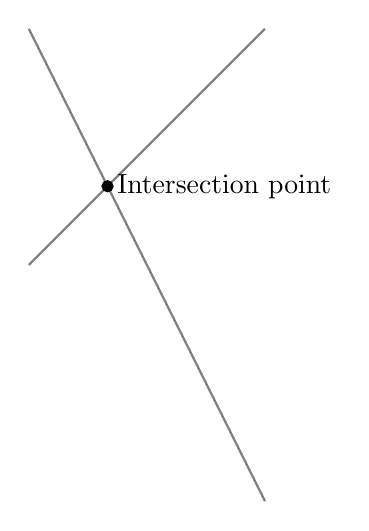
\begin{tikzpicture}
			\draw[gray, thick] (-1,2) -- (2,-4);
			\draw[gray, thick] (-1,-1) -- (2,2);
			\filldraw[black] (0,0) circle (2pt) node[anchor=west]{Intersection point};
		\end{tikzpicture}
	\end{document}
\end{verbatim}
This example produces the following output:
\begin{center}
	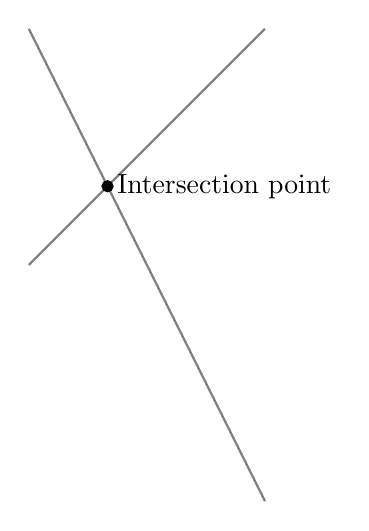
\begin{tikzpicture}
		\draw[gray, thick] (-1,2) -- (2,-4);
		\draw[gray, thick] (-1,-1) -- (2,2);
		\filldraw[black] (0,0) circle (2pt) node[anchor=west]{Intersection point};
	\end{tikzpicture}
\end{center}
In this example 2 lines \& 1 point are drawn. To add a line the command \verb|\draw[gray, thick]| defines a graphic element whose {\it color} is gray \& with a {\tt thick} stroke. The line is actually defined by it's 2 endpoints, {\tt (-1,2)} \& {\tt (2,-4)}, joined by {\tt --}.

The {\it point} is actually a {\tt circle} drawn by \verb|\filldraw[black]|, this command will not only draw the circle but fill it using black. In this command the center point {\tt (0,0)} \& the radius {\tt (2pt)} are declared. Next to the point is a node, which is actually a box containing the text {\tt Intersection point}, \& anchored at the {\tt west} of the point. It's important to notice the semicolon {\tt ;} used at the end of each {\tt draw} command.

\begin{note}
	The {\tt tikzfigure} environment can be enclosed inside a figure or similar environment.''
\end{note}

\subsection{Basic Elements: Points, Lines, \& Paths}
Provide some examples showing how to create some basic graphic elements which can be combined to create more elaborate figures.
\begin{verbatim}
	\documentclass{article}
	\usepackage{tikz}
	\begin{document}
		\begin{tikzpicture}
			
			\draw (-2,0) -- (2,0);
			\filldraw [gray] (0,0) circle (2pt);
			\draw (-2,-2) .. controls (0,0) .. (2,-2);
			\draw (-2,2) .. controls (-1,0) and (1,0) .. (2,2);
			
		\end{tikzpicture}
	\end{document}
\end{verbatim}
This example produces the following output:
\begin{center}
	\begin{tikzpicture}
		
		\draw (-2,0) -- (2,0);
		\filldraw [gray] (0,0) circle (2pt);
		\draw (-2,-2) .. controls (0,0) .. (2,-2);
		\draw (-2,2) .. controls (-1,0) and (1,0) .. (2,2);	
	\end{tikzpicture}
\end{center}
There are 3 basic commands in this example:
\begin{enumerate}
	\item \verb|\draw (-2,0) -- (2,0);|: This defines a line whose endpoints are {\tt (-2,0)} \& {\tt (2,0)}.
	\item \verb|\filldraw [gray] (0,0) circle (2pt);|: The point is created as a very small {\tt gray circle} centered at {\tt (0,0)} \& whose radius is {\tt (2pt)}. The \verb|\filldraw| command is used to draw elements \& fill them with a specific color.
	\item \verb|\draw (-2,2) .. controls (-1,0) and (1,0) .. (2,2);|: Draw a \href{https://en.wikipedia.org/wiki/B%C3%A9zier_curve}{B\'ezier curve}. There are 4 points defining it: {\tt (-2,2)} \& {\tt (2,2)} are its endpoints, {\tt (-1,0)} \& {\tt (1,0)} are \href{https://en.wikipedia.org/wiki/Control_point_(mathematics)}{{\it control points}} that determine ``how curved'' it is. You can think of these 2 points as ``attractor points''.''
\end{enumerate}

\subsection{Basic Geometric Shapes: Circles, Ellipses, \& Polygons}
``Geometric figures can be constructed from simpler elements so let's start with circles, ellipses, \& arcs.
\begin{verbatim}
	\documentclass{article}
	\usepackage{tikz}
	\begin{document}
		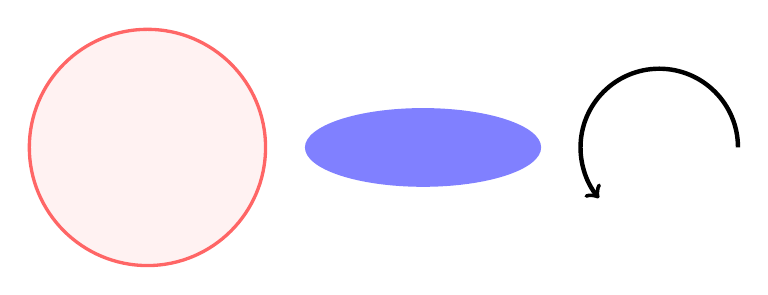
\begin{tikzpicture}
			\filldraw[color=red!60, fill=red!5, very thick](-1,0) circle (1.5);
			\fill[blue!50] (2.5,0) ellipse (1.5 and 0.5);
			\draw[ultra thick, ->] (6.5,0) arc (0:220:1);
		\end{tikzpicture}
	\end{document}
\end{verbatim}
This example produces the following output:
\begin{center}
	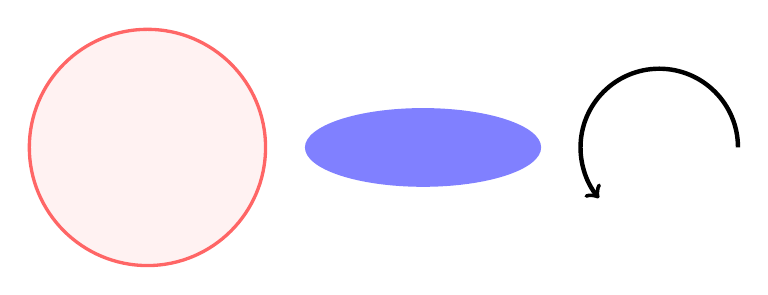
\begin{tikzpicture}
		\filldraw[color=red!60, fill=red!5, very thick](-1,0) circle (1.5);
		\fill[blue!50] (2.5,0) ellipse (1.5 and 0.5);
		\draw[ultra thick, ->] (6.5,0) arc (0:220:1);
	\end{tikzpicture}
\end{center}
\begin{enumerate}
	\item \verb|\filldraw[color=red!60, fill=red!5, very thick](-1,0) circle (1.5);|: This command was used in the previous section to draw a {\it point}, but in this instance there are some additional parameters inside the brackets. These are explained below:
\end{enumerate}

\subsection{Diagrams}

%------------------------------------------------------------------------------%

\section{\href{https://www.overleaf.com/learn/latex/Typesetting_quotations}{Overleaf{\tt /}typesetting quotations}}

\subsection{Introduction}
``When it comes to quotations \& quotation marks, each language has its own symbols \& rules. 

\subsection{{\tt dirtytalk} package}

\subsection{{\tt csquotes} package}

\subsection{{\tt epigraph} package}

\subsection{{\tt fancychapters} package (obsolete)}

\subsection{{\tt quotchap} package}

\subsection{Reference guide}

%------------------------------------------------------------------------------%

\section{Vanilla \TeX Live}
\textsc{Ubuntu} does not pre-install Vanilla \TeX Live, you need to install it manually \& additionally.

%------------------------------------------------------------------------------%

\printbibliography[heading=bibintoc]
	
\end{document}